\documentclass[12pt]{amsart}
\usepackage[margin=1.1in]{geometry}
\usepackage{graphicx}
\linespread{1.0}
\newcommand{\ZZ}{\mathbb{Z}}
\newcommand{\QQ}{\mathbb{Q}}
\newcommand{\RR}{\mathbb{R}}
\newcommand{\CC}{\mathbb{C}}
\newcommand{\HH}{\mathbb{H}}
\newcommand{\FF}{\mathbb{F}}

\newcommand{\rank}{\mathop\mathrm{rank}}
\newcommand{\supp}{\mathop\mathrm{supp}}
\newcommand{\tr}{\mathop\mathrm{tr}}
\newcommand{\Span}{\mathop\mathrm{span}}

\newcommand{\cl}[1]{\overline{#1}}
\newcommand{\Id}{\mathop\mathrm{Id}}
\newcommand{\Int}{\mathop\mathrm{int}}

\newcommand{\Exercise}[1]{\ \par\noindent\textbf{\em{[#1]}}\\}
\newcommand{\Subexe}[1]{\ \par\noindent\textbf{\em{(#1).}}~}
\newcommand{\Subsubexe}[1]{\ \par\indent\emph{(#1).}~}

\makeatletter
\renewcommand{\section}{\@startsection{section}{1}{0mm}
{-\baselineskip}{0.5\baselineskip}{\bf\leftline}}
\makeatother

\begin{document}
\noindent Machine Learning \hfill Jiecao Chen \hfill ID:4716311 \\
\textsc{Homework \#1}\\



%%%%%%%%%%%%%%%%%%%%%%%%%%%%%%%%%%%%%%%%%%%%%%%%%%%%%%%%%%%%%
\section*{Question 1} 
\subsection*{a}
\begin{align*}
	E[\mathfrak{l}(f(x), y)] 
	&= \int\int (f(x) - y)^2 p(x, y) dxdy\\
	&= \int\int
		\{ (f(x) - E[y|x])^2 + (y - E[y|x])^2 +
	 	 2(f(x) - E[y|x]) (y - E[y|x]) \} p(x, y) dxdy					
\end{align*}
note that $E[y|x]$ is a function of $x$, thus
$$
	\int\int 2(f(x) - E[y|x]) (y - E[y|x]) p(x, y) dxdy	=
	\int 2(f(x) - E[y|x]) (E[y|x] - E[y|x]) p(x) dx =
	0	
$$
so we have 
\begin{align*}
	E[\mathfrak{l}(f(x), y)]  = 
	\int\int
		\{ (f(x) - E[y|x])^2 + (y - E[y|x])^2
	 	\} p(x, y) dxdy	\geq \int\int  (y - E[y|x])^2 p(x, y) dxdy
\end{align*}
to minimize it, simply let $f(x) = E[y|x]$

\subsection*{b}
our goal is to minimize
\begin{align*}
	E[\mathfrak{l}(f(x), y)]  
	&=	\int\int |f(x) - y| p(x, y) dx dy\\
	&=	\int (\int |f(x) - y| p(y|x)	dy) p(x)dx	
\end{align*}
as for every $x$, the value of $f(x)$ could be independently chosen, 
thus we just need to minimize
$$
	\int |f(x) - y| p(y|x)	dy
$$
now calculate the derivative of above expression with respect to $f(x)$, and set
it to zero, we have
\begin{align*}
	0 = \int sign( f(x) - y ) p(y|x) dy 
	&= \int_{f(x)}^{+\infty} p(y|x) dy - \int^{f(x)}_{-\infty} p(y|x) dy\\	
\end{align*}
which implies 
$$
	\int_{f(x)}^{+\infty} p(y|x) dy = \int^{f(x)}_{-\infty} p(y|x) dy
$$
which is the condition $f(x)$ must satisfy to minimize $E[\mathfrak{l}(f(x), y)]$




%%%%%%%%%%%%%%%%%%%%%%%%%%%%%%%%%%%%%%%%%%%%%%%%%%%%%%%%%%%
\section*{Question 2}
let's try to minimize
\begin{align*}
	L(f) = P(f(x) \neq y) 
	&= \int\int \mathbf{1}(f(x)\neq y ) p(x, y) dxdy\\
	&= \int \big ( \int \mathbf{1}(f(x)\neq y ) p(y|x) dy \big ) p(x) dx
\end{align*}
as $f(x)$ could independently chosen for every $x$, thus we just need to minimize
$$
	\int \mathbf{1}(f(x)\neq y ) p(y|x) dy 
	=  \mathbf{1}(f(x) \neq 1 ) P(1|x) + \mathbf{1}(f(x) \neq 0 ) P(0|x) = (1)
$$
let's discuss how to set $f(x)$ to minimize (1)
\begin{itemize}
\item case 1: $P(1|x) > 1/2, P(0|x) = 1 - P(1|x) < 1/2$, \\
				should choose $\mathbf{1}(f(x) \neq 1 )  = 1$ and
				$\mathbf{1}(f(x) \neq 0 ) = 0$ to minimize (1)
\item case 2: $P(1|x) < 1/2, P(0|x) = 1 - P(1|x) > 1/2$, \\
				should choose $\mathbf{1}(f(x) \neq 1 )  = 0$ and
				$\mathbf{1}(f(x) \neq 0 ) = 1$ to minimize (1)
\item case 3: $P(1|x) = P(0|x) = 1/2$,\\
				any assignment for $\mathbf{1}(f(x) \neq 1 )$ and $\mathbf{1}(f(x) \neq 0 )$
				is OK
\end{itemize}

we note that $f^*(x)$ satifies above discussion thus is an optimal solution for 
$$
	minimize~~:~~L(f) 
$$
so we have proved $L(f) \geq L(f^*)$


%%%%%%%%%%%%%%%%%%%%%%%%%%%%%%%%%%%%%%%%%%%%%
\section*{Question 3}
\subsection*{Fisher's Linear Discriminant}
\subsubsection*{Idea}
The main idea of \textbf{Fisher's Linear Discriminant} is to project the
features from a high-dimention space to a low-dimention space when maximize the 
distinctions between different classes.  And Fisher set the criterion as
$$
	J(w) = \frac{w^TS_Bw}{w^TS_Ww}
$$
the value of $J(w)$ indicates the distance between different classes.
To get the optimal $w$, we just need to select the $D'$ largest eigenvalues of $S_W^{-1}S_B$ where $D'$ is the dimention of the projected feature space.
In the code \textbf{diagFisher}, we simply set $S_w = I$.
\subsubsection*{Experiment results}
In our implementatin, the dimention of projected feature space $D'$ was set as $3$ for
data "Iris.csv" and $9$ for "Wine.csv", and in the projected space, \textbf{Gaussian Generative Model} will be used to do classification\\
================================


\begin{verbatim}
$ python diagFisher.py 'Iris.csv' 10

Data:  Iris.csv
Error rate for cross_validation: 0.0333333333333

$ python Fisher.py 'Iris.csv' 10

Data:  Iris.csv
Error rate for cross_validation: 0.02

$ python diagFisher.py 'Wine.csv' 10

Data:  Wine.csv
Error rate for cross_validation: 0.0588235294118


$ python Fisher.py 'Wine.csv' 10

Data:  Wine.csv
Error rate for cross_validation: 0.0470588235294
\end{verbatim}
=================================

we can see that both models are quite accurate, and the performence of $Fisher.py$ is 
slightly better.



\subsection*{Least squares linear discriminant}
\subsection*{Idea}
This model is quite simple and we just need to minimize the following criterion
$$
	E(W) = \frac{1}{2}Tr\big \{ (Y - XW)^T (Y-XW) \big \}
$$
The optimal solution would be
$$
	W = (X^TX)^{-1}X^TY
$$
where $X$ is the matrix of features and $Y$ is the vector of labels.

\subsection*{Experiment results}
let's see our result\\
================================
\begin{verbatim}
$ python SqClass.py 'Iris.csv' 10
Data:  Iris.csv
Error rate for cross_validation: 0.2

$ python SqClass.py 'Wine.csv' 10
Data:  Wine.csv
Error rate for cross_validation: 0.0235294117647
\end{verbatim}
=================================

much worse than \textbf{Fisher's} method for data 'Iris.csv', 
but better for 'Wine.csv'




\section*{Question 4}
\subsection*{i}
\subsubsection*{Idea}
\textbf{Logistic regression} assume that
$$
	log(\frac{P(C_h|\phi)}{P(C_k|\phi)}) = W^T\phi + W_0
$$
then we want to minimize the negative log-likeihood
$$
	E(W) = -\Sigma_{n=1}^N \big \{ y_nW^t\phi_n - log(1 + exp(W^T\phi_n)) \big \}
$$
The gradient of the objective function
$$
\nabla E(W) = \phi^T (\pi - y)
$$
The using the Newton-Raphson iterative optimization
$$
W^{new} = W^{old} - H^{-1}(W^{old}) \nabla E(W^{old})
$$

\subsubsection*{Result}
See
\ref{fig:verticalcell1}
\ref{fig:verticalcell2}
\ref{fig:verticalcell3}
\ref{fig:verticalcell4}

\begin{figure}[H]
\centering
        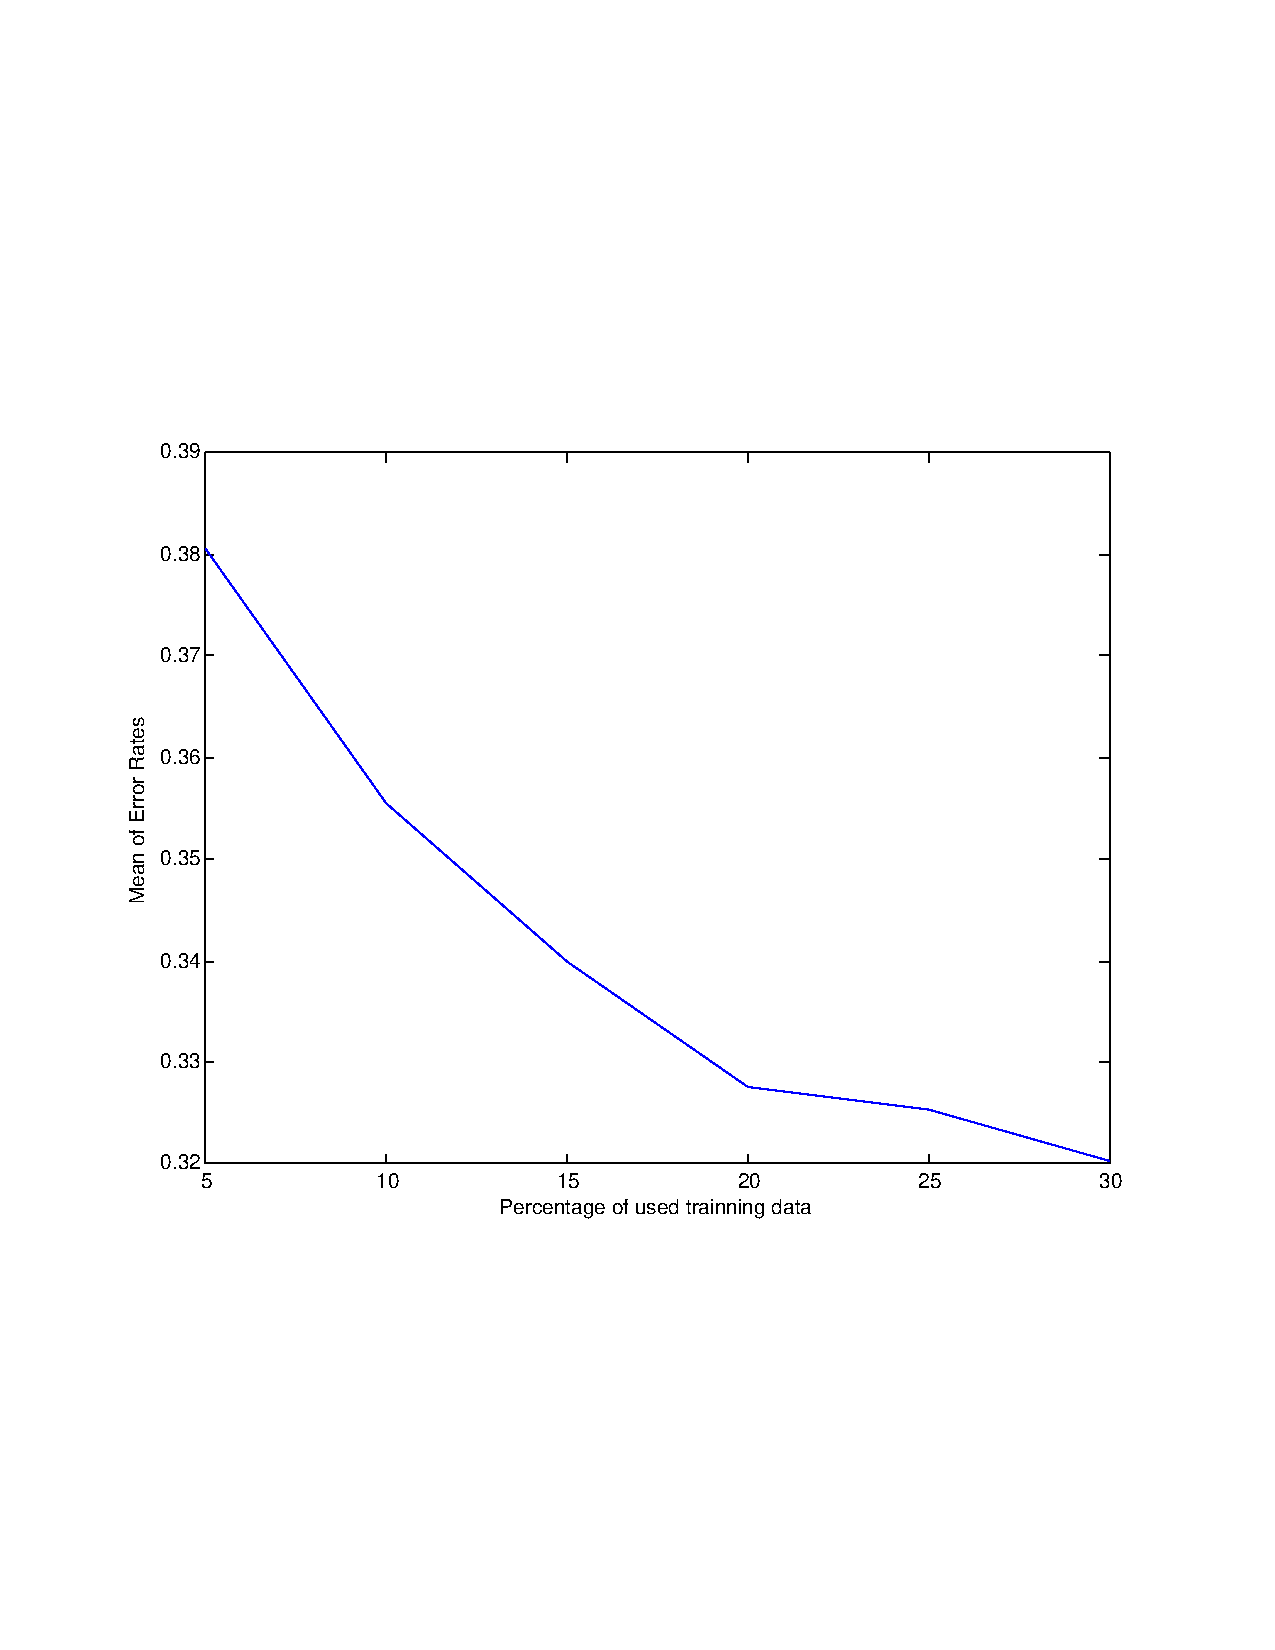
\includegraphics[totalheight=18cm]{Pima_mean_rogReg.pdf}
    \caption{mean of error rates for Pima.csv}
    \label{fig:verticalcell1}
\end{figure}

\begin{figure}[H]
\centering
        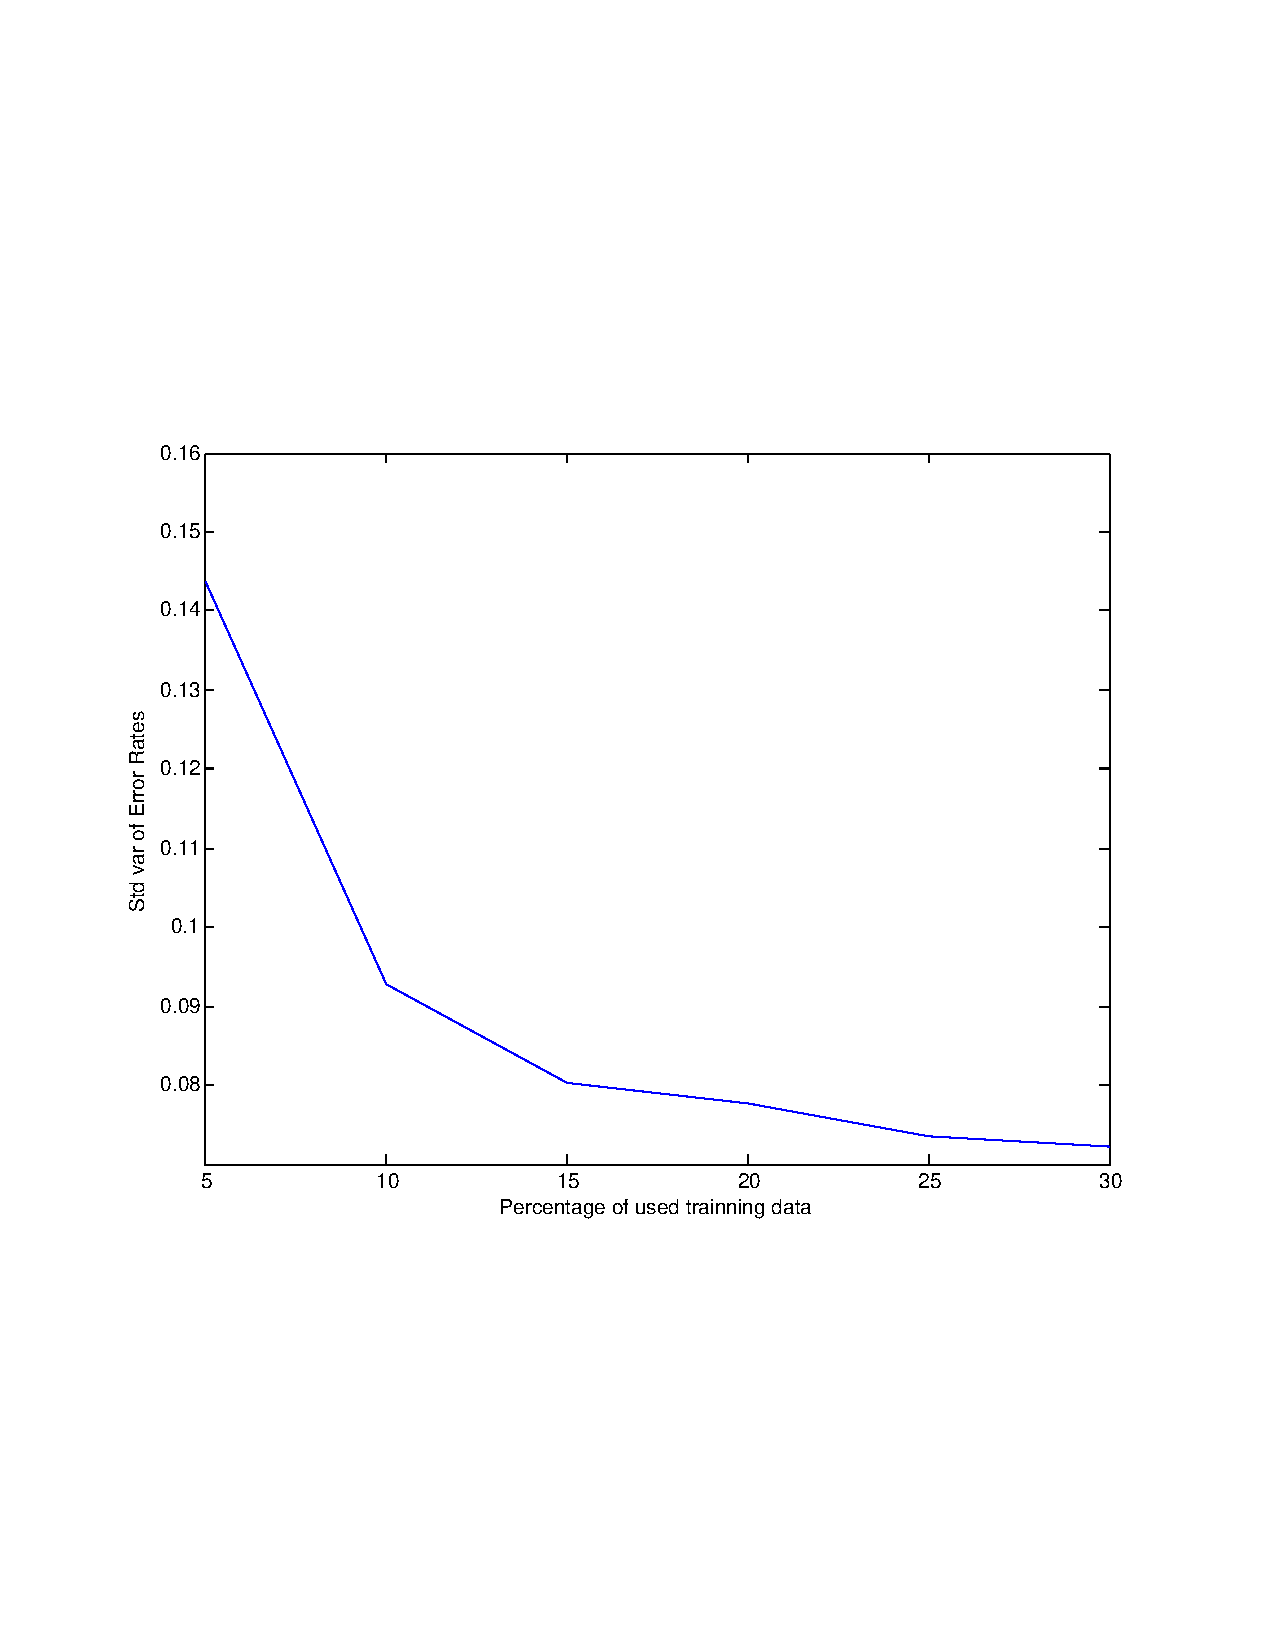
\includegraphics[totalheight=18cm]{Pima_std_rogReg.pdf}
    \caption{standard var of error rates for Pima.csv}
    \label{fig:verticalcell2}
\end{figure}

\begin{figure}[H]
\centering
        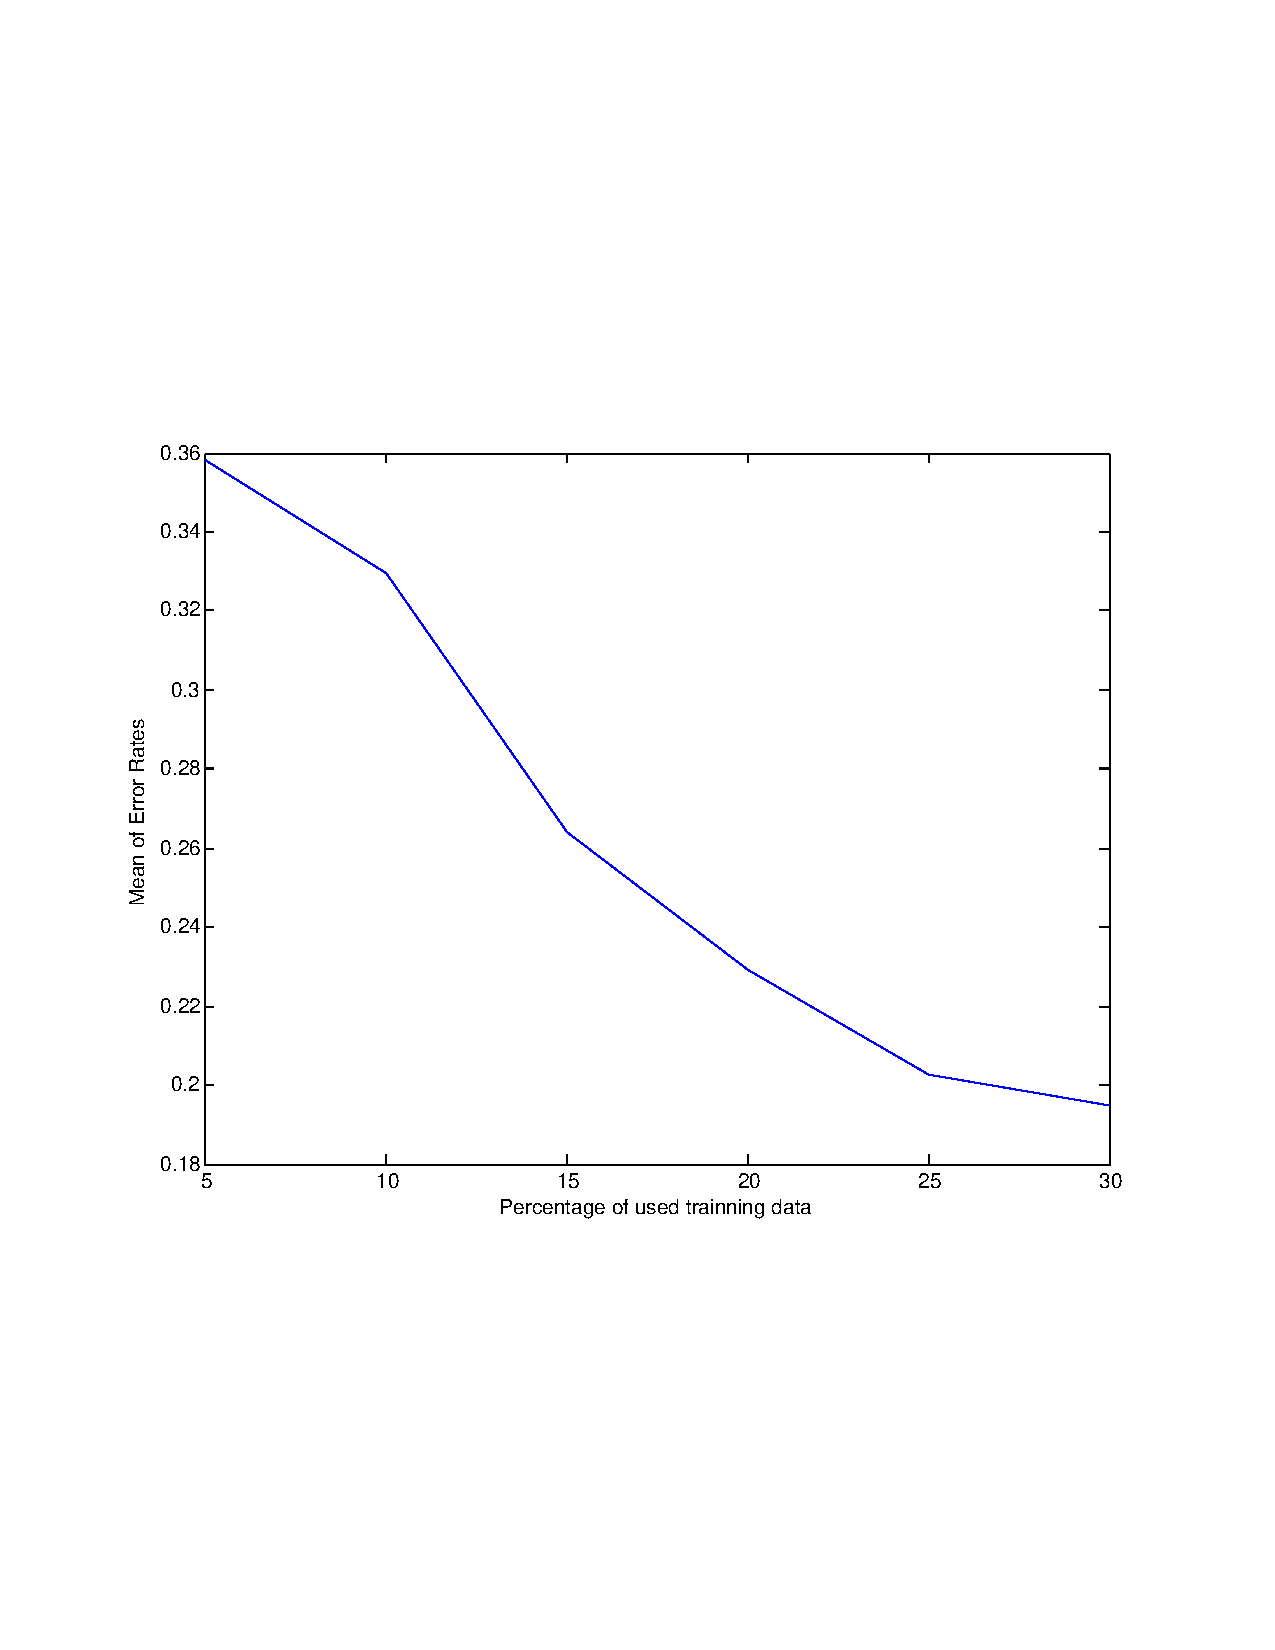
\includegraphics[totalheight=18cm]{Iono_mean_logReg.pdf}
    \caption{mean of error rates for Ionosphere.csv}
    \label{fig:verticalcell3}
\end{figure}

\begin{figure}[H]
\centering
        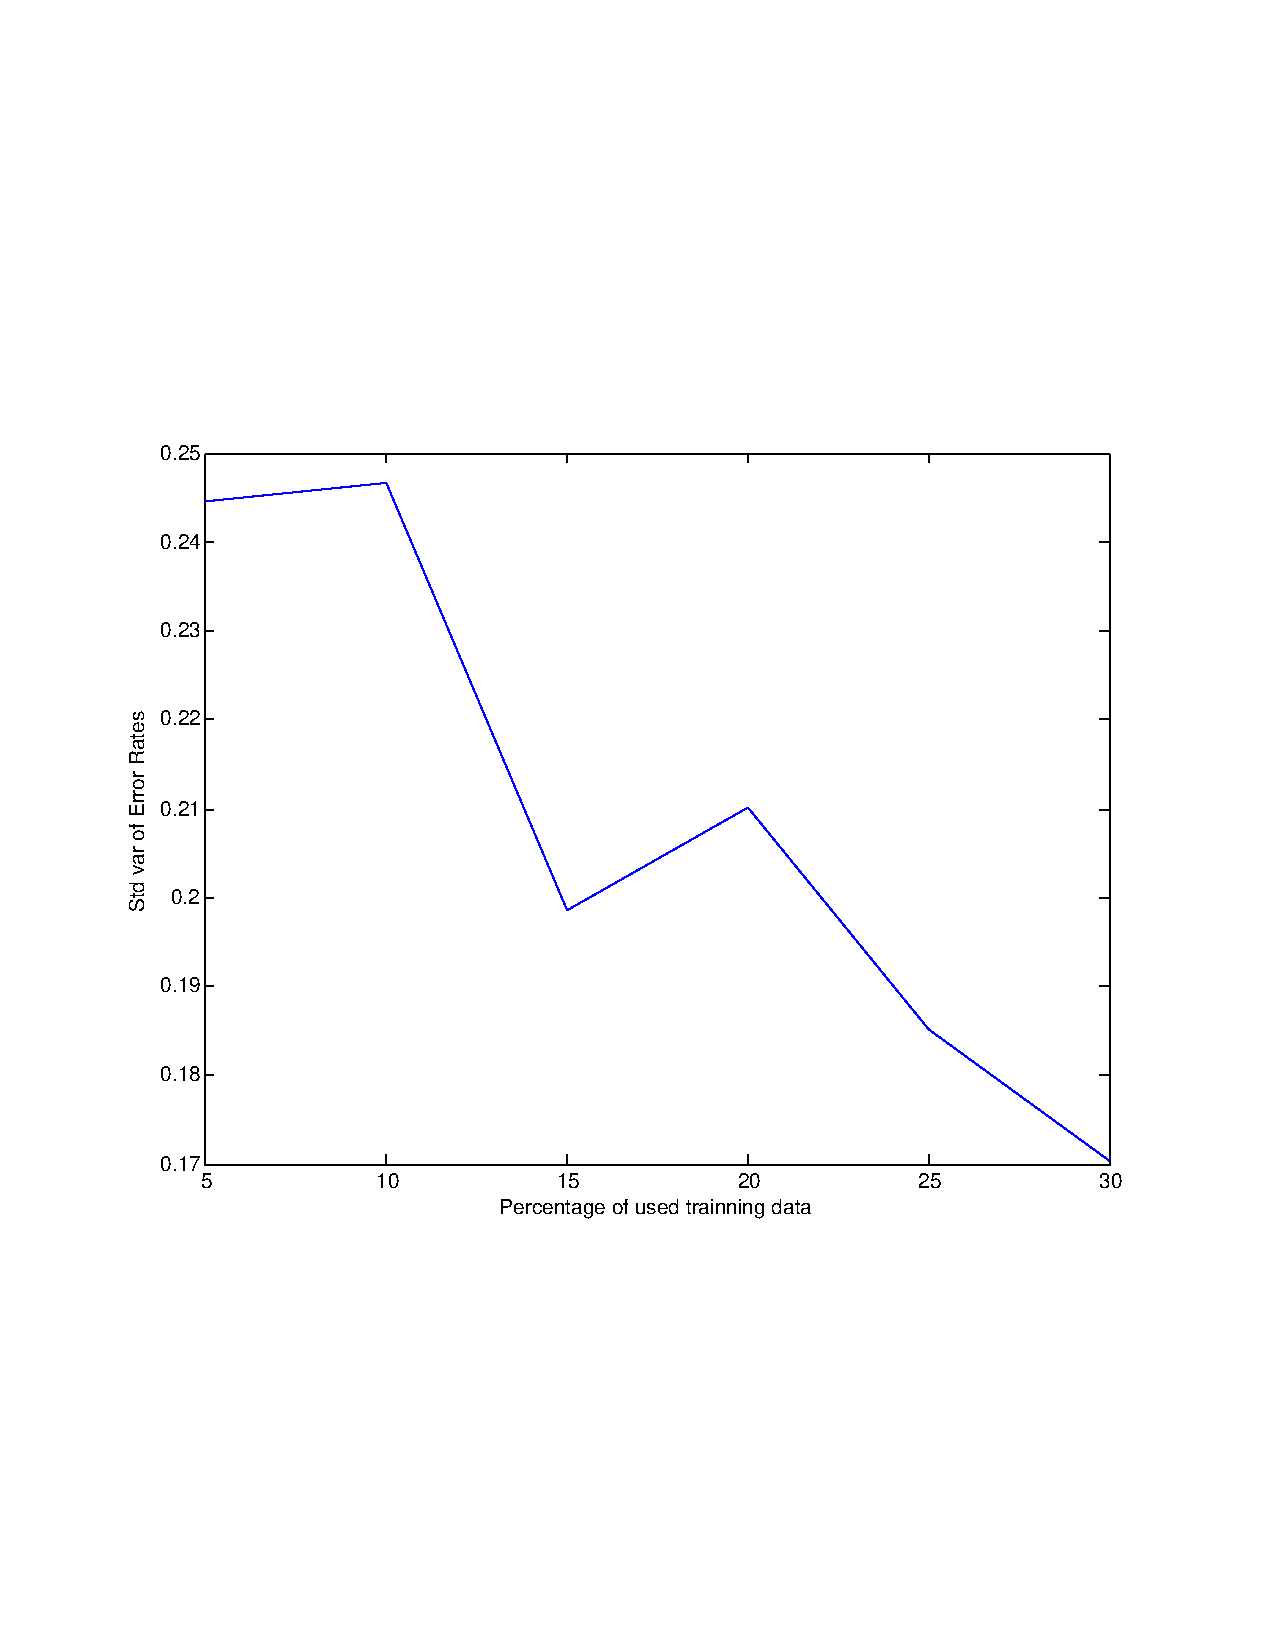
\includegraphics[totalheight=18cm]{Iono_std_logReg.pdf}
    \caption{standard var of error rates for Ionosphere.csv}
    \label{fig:verticalcell4}
\end{figure}
\subsection*{ii}
\subsubsection*{Idea}
\textbf{Naive Bayes Gaussian} assumes features are independent and
class conditionals $p(x|C_k)$ are Gaussian

for K-class problem
$$
	a_k(x) = \sigma(w_k^Tx + w_{k0})
$$
$$
	w_k = \Sigma^{-1}\mu_k\\
	w_{k0} = \frac{1}{2}\mu_k^T \Sigma^{-1}\mu_k + log p(C_k)
$$

\subsubsection*{Result}
See
\ref{fig:verticalcell11}
\ref{fig:verticalcell21}
\ref{fig:verticalcell31}
\ref{fig:verticalcell41}

\begin{figure}[H]
\centering
        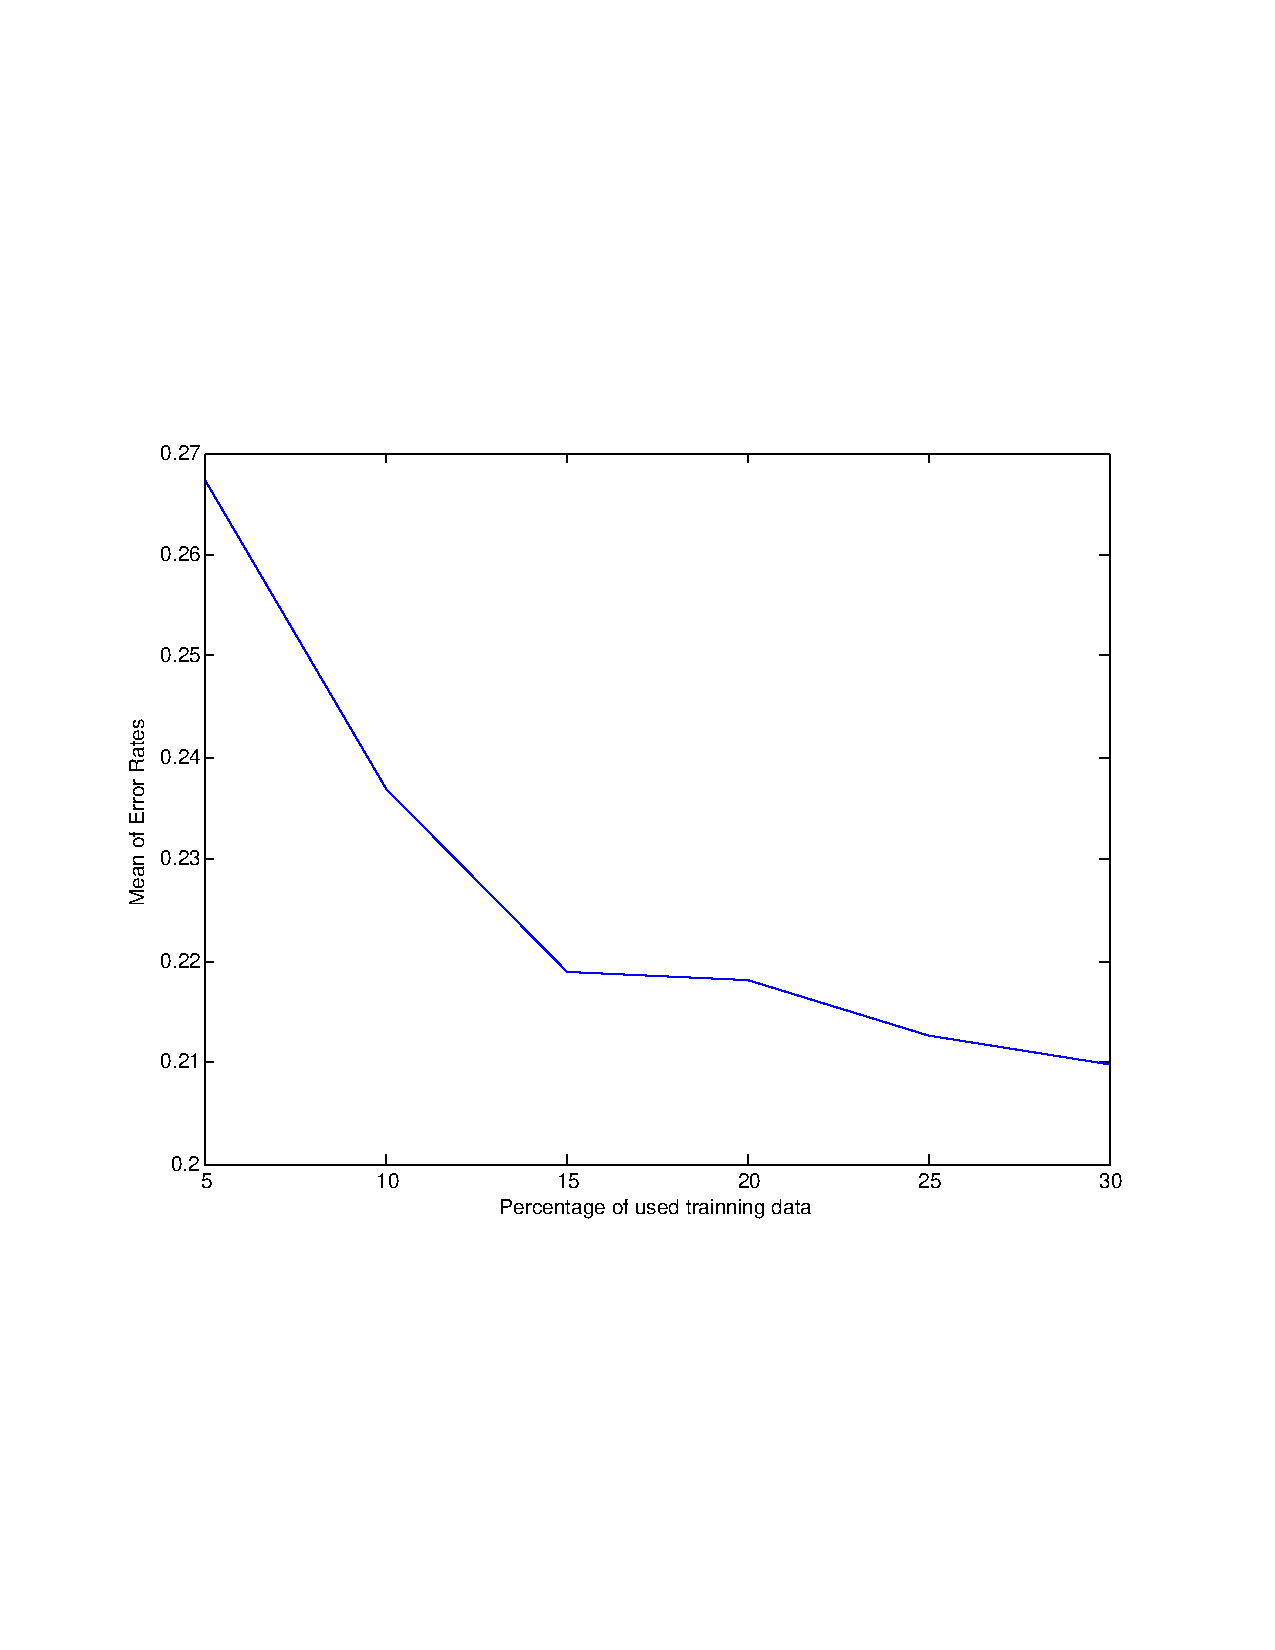
\includegraphics[totalheight=18cm]{Pima_mean_nbg.pdf}
    \caption{mean of error rates for Pima.csv}
    \label{fig:verticalcell11}
\end{figure}

\begin{figure}[H]
\centering
        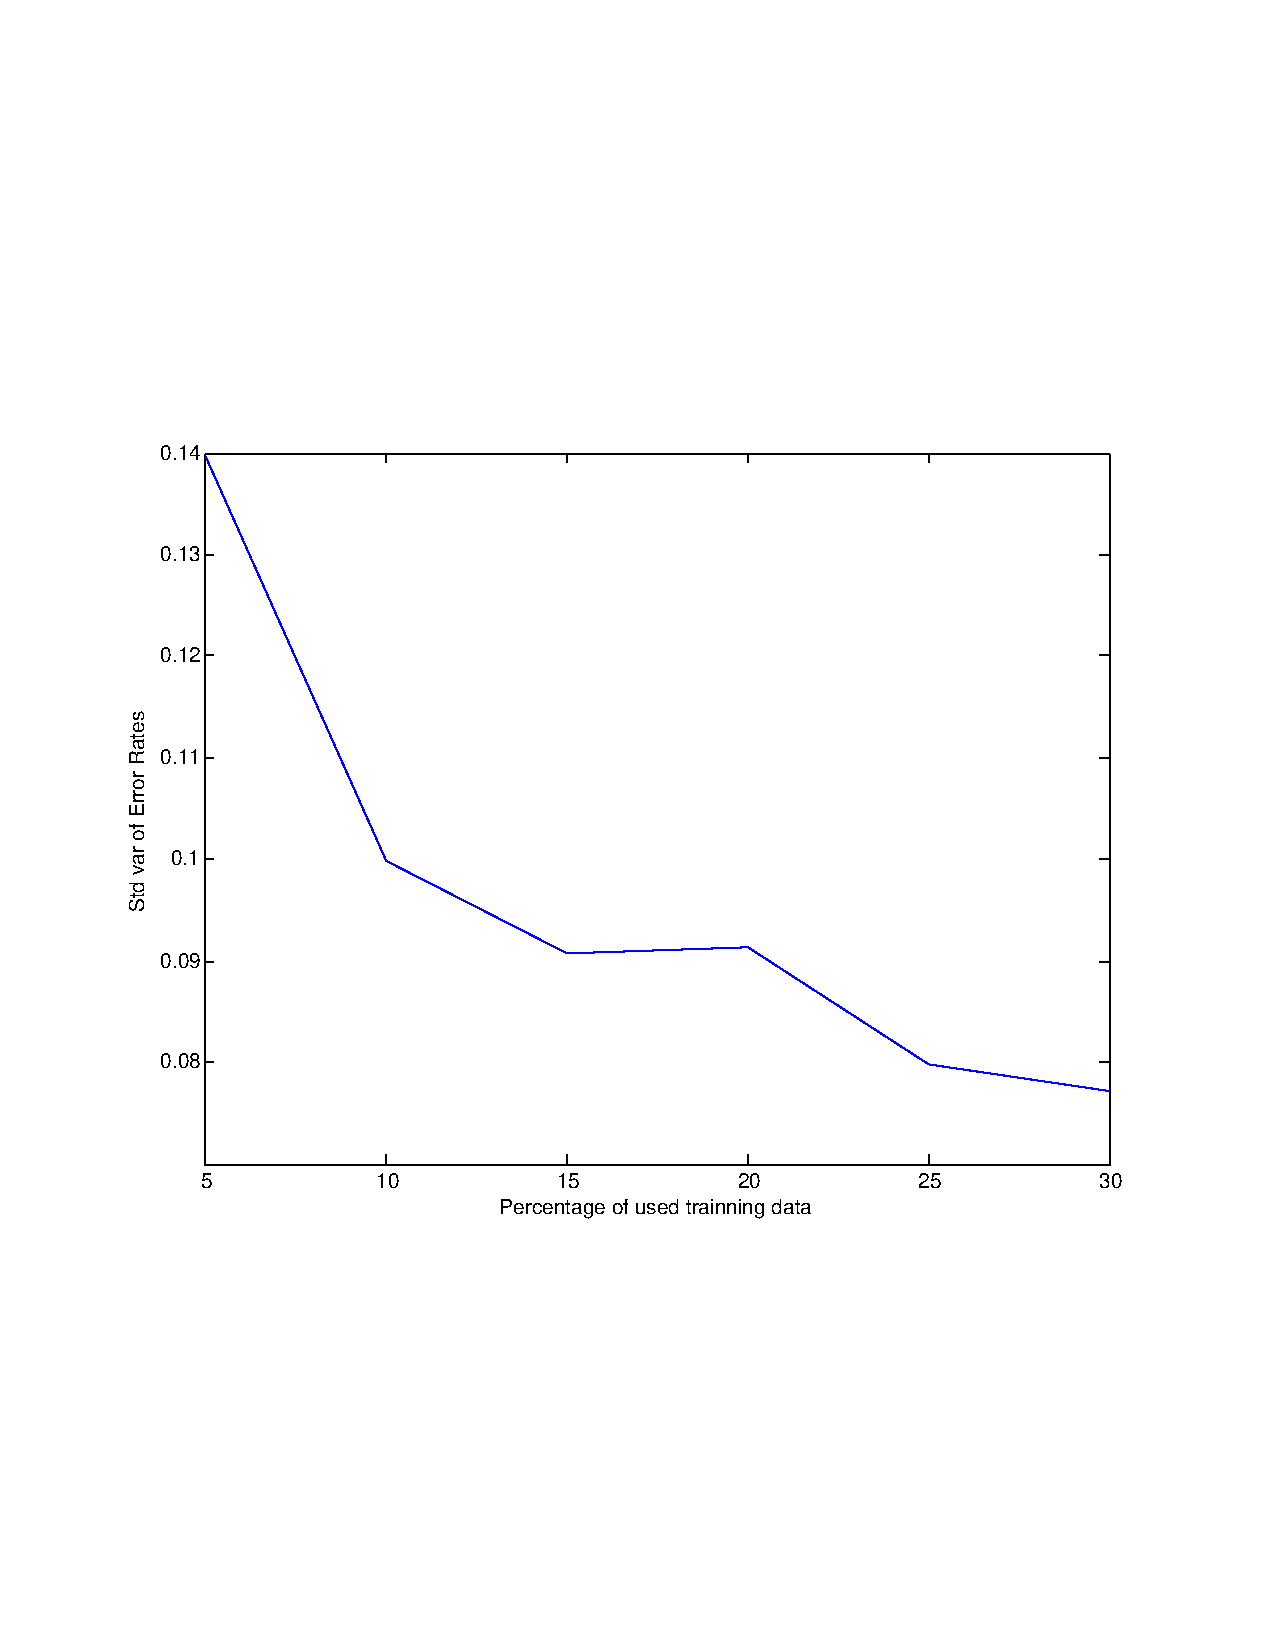
\includegraphics[totalheight=18cm]{Pima_std_nbg.pdf}
    \caption{standard var of error rates for Pima.csv}
    \label{fig:verticalcell21}
\end{figure}

\begin{figure}[H]
\centering
        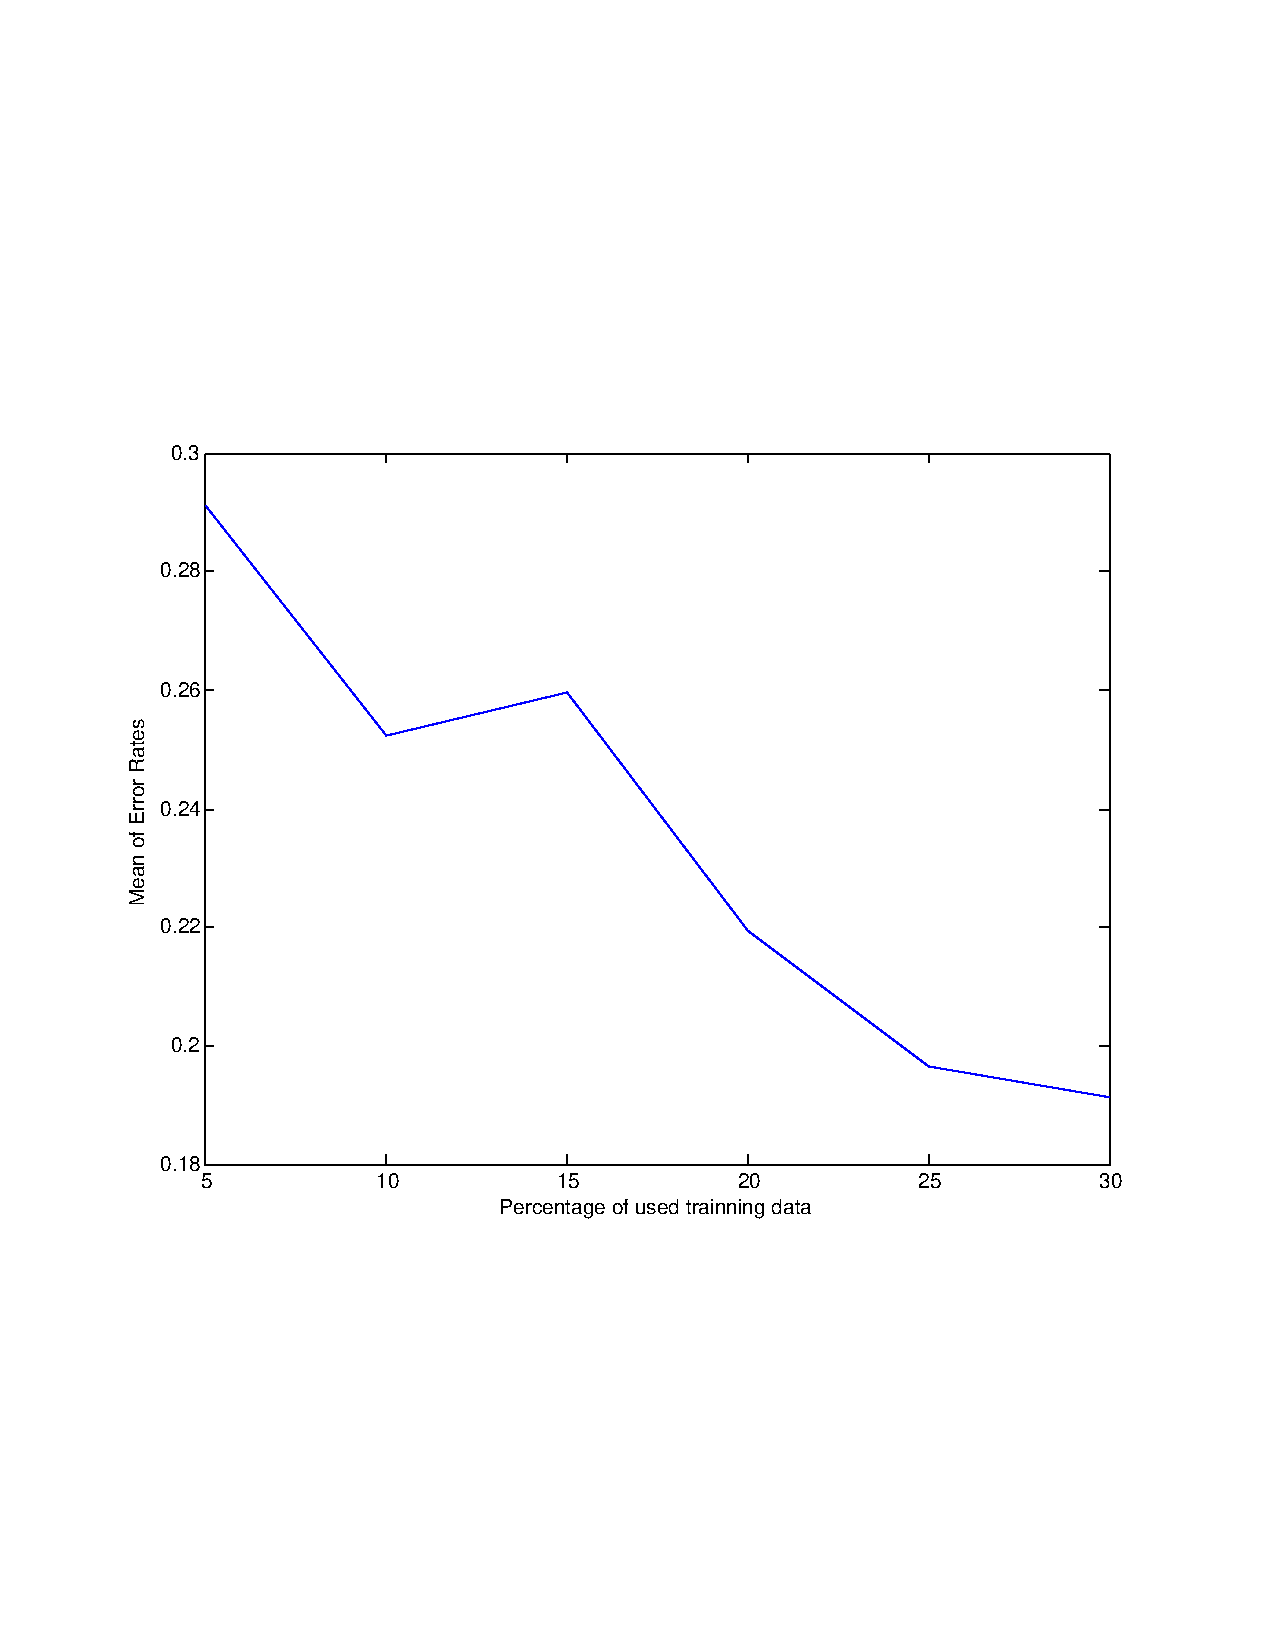
\includegraphics[totalheight=18cm]{Iono_mean_nbg.pdf}
    \caption{mean of error rates for Ionosphere.csv}
    \label{fig:verticalcell31}
\end{figure}

\begin{figure}[H]
\centering
        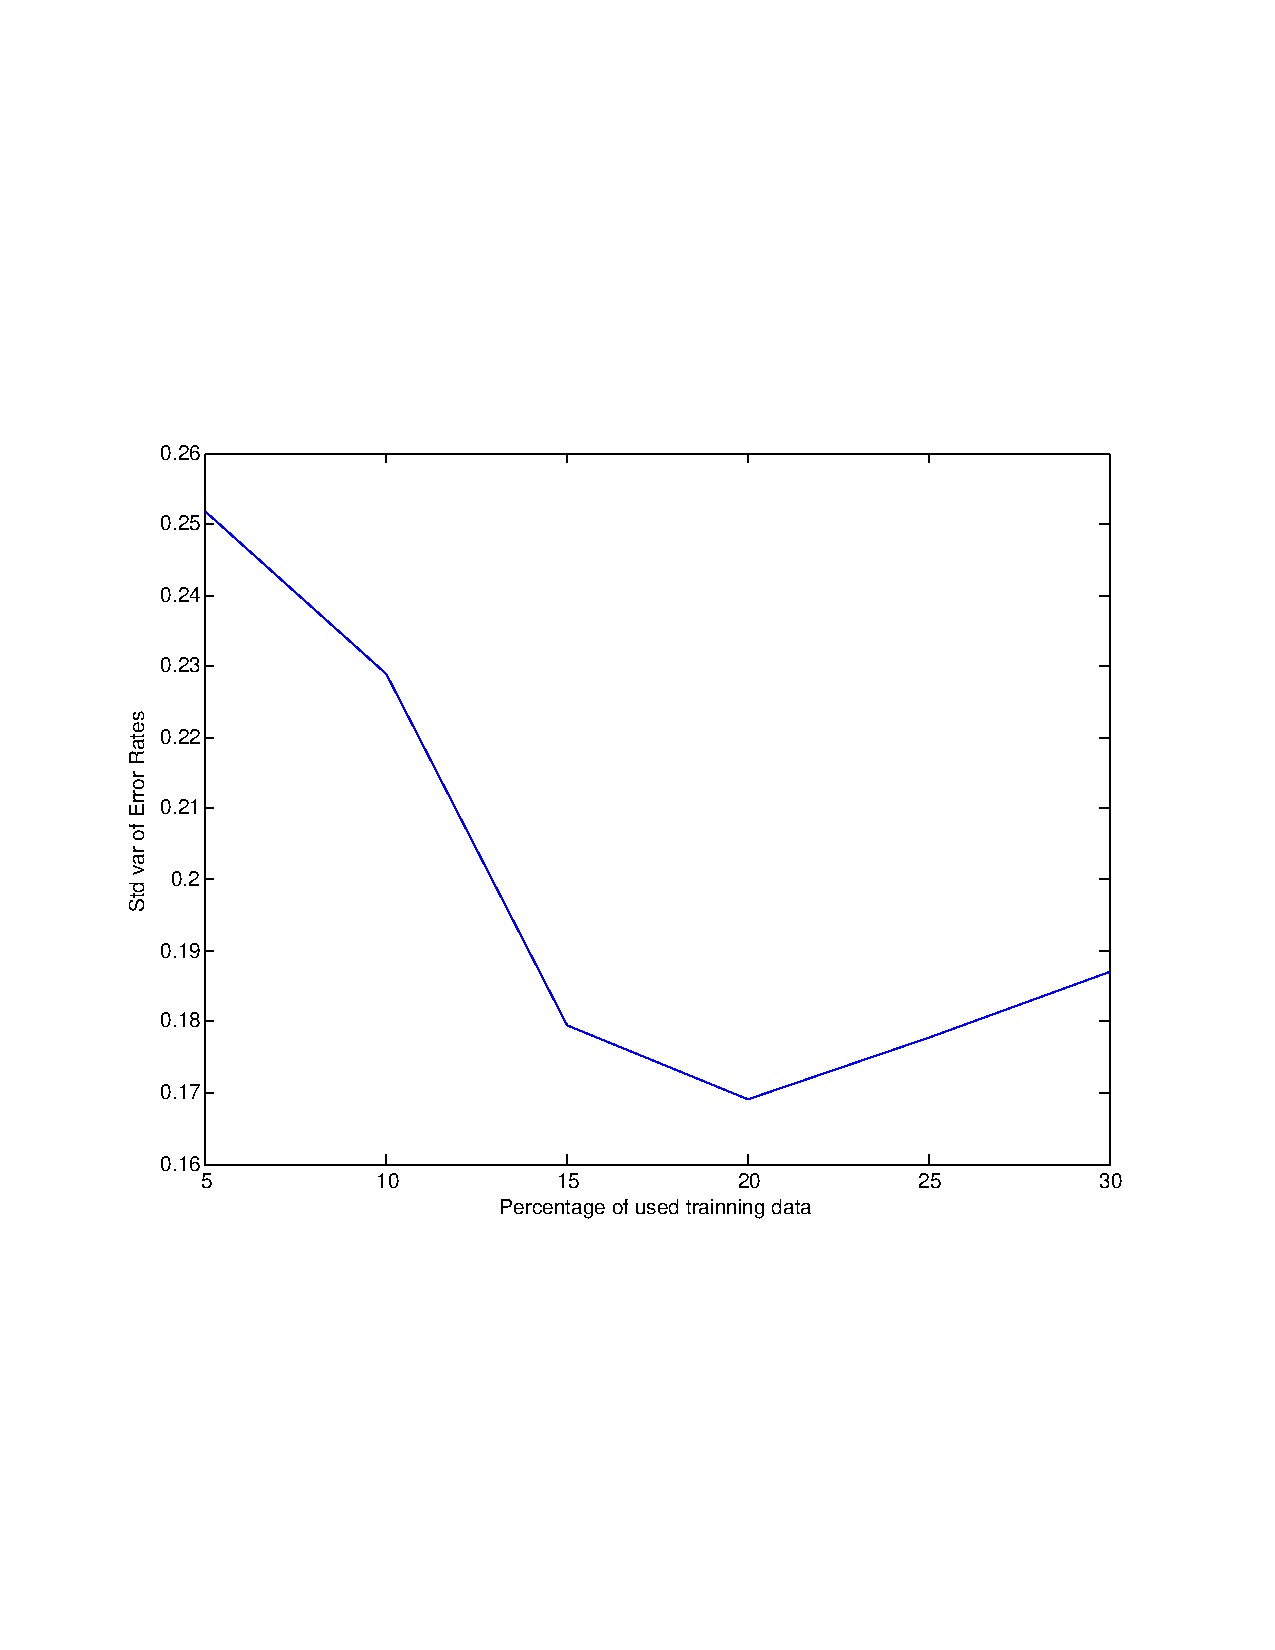
\includegraphics[totalheight=18cm]{Iono_std_nbg.pdf}
    \caption{standard var of error rates for Ionosphere.csv}
    \label{fig:verticalcell41}
\end{figure}
\end{document} 
